\chapter{Design}

\section{Compiler Support}

There are several broad approaches to implementing an AOP framework. I believe the ideal approach would be to extend the compiler of the target language to provide built-in support, making AOP the first class citizen. However there are very few languages out there that take this approach, such as Delphi Prism~\cite{delphi_prism2010} and AspectJ~\cite{aspectj_faq, aspectj_text}. 

Microsoft is in the "wait and see" mode regarding support of AOP development in the C\# compiler~\cite{hejlsberg}. Which means it is unlikely to happen anytime soon. Alternative compiler such as Mono C\#~\cite{monocsharp} is open source, so technically anyone can build AOP support into it. However that would have been a fairly big undertaking, and I was not sure if I can tackle and finish it in the time frame I wanted.

That leaves framework support as the other viable option. There are several implementation techniques to provide AOP capabilities~\cite{aopcs, postsharp, aspectcs}.

\section{Run-time Interception}

Early on I have narrowed them down to between Run-time Interception and Compile Time Weaving. As its name suggested, run-time interception operates while the program is in execution. It involves the use of the proxy pattern, where client communicate with the target object via a proxy, and aspects are injected to the proxy, thus enabling run-time behavior of the program to be modified. Figure~\ref{proxy_model} illustrates this process.

\begin{figure}[H]
  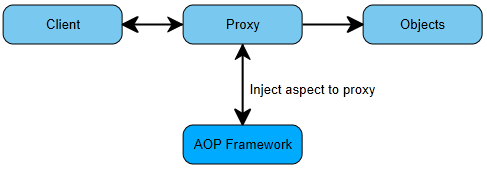
\includegraphics[scale=1.0]{Proxy.PNG}
  \centering
  \caption{AOP Framework Using Proxy Pattern\label{proxy_model}}
\end{figure}

New functionality can be “added” to the target object via the proxy. The disadvantage of this approach is that it involves the generation of proxy object at run-time, which will impact the run-time performance of the application. It is also restricting in that both target object and the proxy must implement a common interface for this to work, and that only virtual methods are exposed for interception.

From the end user's perspective, to use it the developer usually have to provide some type of mapping between the target object and the proxy via a configuration file so the actual proxy generation can occur. This approach although is easier to implement, but not as easy and friendly to use.

\section{Compile Time Weaving}

The approach Buffalo takes is Compile Time Weaving. The basic idea is after compilation of the assembly, the framework takes over and disassembles the assembly. Buffalo then weaves in the defined aspect code to all targeted methods. This approach is more difficult to implement as it involves modifying the underlying assembly by changing Common Intermediate Language (CIL) instructions~\cite{rewrite_msil}. But the advantage is that no run-time performance of proxy generation will be needed. And since this happens post-compilation we can hook it into the Microsoft Build System to have the weaving invoked automatically if needed, so no manual setup is required from the developer.

Figure~\ref{buffalo_model} shows an overview of the compilation process and where Buffalo will fit in.

\begin{figure}[H]
  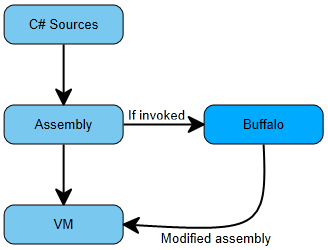
\includegraphics[scale=1.0]{BuffaloOverview.PNG}
  \centering
  \caption{Buffalo Model\label{buffalo_model}}
\end{figure}

\section{What is a Buffalo Aspect}

When performing post compilation weaving, Buffalo has to be able to discover what aspect is applied to what method in an assembly. In order to achieve that the target assembly has to carry some extra meta-data, so that Buffalo can use that to identify aspects.

A given .NET assembly already carries a great deal of such meta-data for various purpose. .NET has the System.Attribute type that exists primarily for the purpose of inserting meta-data into the assembly during compilation. When we compile the source code, it is converted into CIL~\cite{msil_text} and put inside a portable executable (PE) file, with the meta-data generated by the compiler. Buffalo takes advantage of this characteristic in two areas.

First, an aspect defined in Buffalo will be in the form of an attribute, by sub-classing System.Attribute. Since the aspect is a class type, it can contains any valid .NET code. But specifically an aspect needs to override various predefined methods in order to do something useful. To see a detail relationship between various aspect types, please refer to figure~\ref{uml01}.

Second, after compilation, the assembly will now contain the meta-data about the aspect. Buffalo can inspect the assembly for the information, and perform CIL code injection accordingly.

In other word, a Buffalo aspect is a .NET attribute in disguise.

\section{MethodBoundaryAspect}
I also have to decide on what functionality I want to support in the framework. What type of aspects do I want to weave into the IL instructions of the executing program? For this I took inspiration from AspectJ~\cite{aspectj_faq} and PostSharp~\cite{postsharp}, specifically I want to intercept the various point of an executing method. Those points are namely: before a method executes; after a method executes; whether or not the method executed successfully without error; or whether the method throws an exception any point during the execution.

If we think about it, these points can be cleanly mapped to the try-catch-finally statements of the .NET languages. As far as the run-time is concern~\cite{ecma334, ecma335}, try-catch can be used liberally without serious performance degradation. For example, we can transform the following method:

\begin{lstlisting}[caption={Sample function}, label=samplefunction]
public void SomeFunction () {
   //Perform some action...
}
\end{lstlisting}

With something like the following, which will capture exactly what I have in mind:

\begin{lstlisting}[caption={Sample try-catch-finally}, label=sampletcf]
public void SomeFunction () {
   try {
       OnBefore();
       //Perform some action
       OnSuccess();
   }
   catch (Exception e) {
       OnException(e);
   }
   finally {
       OnAfter();
   }
}
\end{lstlisting}

The above transformed method still does what the original method intends to do, only now at various point execution are being intercepted. I call these various point of interception the MethodBoundaryAspect.

\section{MethodAroundAspect}
Another type of aspect that Buffalo implemented is the MethodAroundAspect. Rather than intercepting various execution point, I can also completely replace a target method with some other method defined in an aspect. While preserving the option to call back into the original method if necessary.

At first glance MethodAroundAspect sounds straightforward to do, but it turns out to be much more involved than the MethodBoundaryAspect.

Since the option to call back into the original method is preserved, that means I should under no circumstance modify the original method. If I simply yank out its method body instructions and replace them with my own, the call back to the original method will be meaningless since the method is changed. The original method must be intact for the call back to happen.

This leads me to dynamically generating a method in CIL with the same method signature as the original.

In this generated method I issued a call to the aspect’s Invoke() method, which is the actual aspect code I want to run. Inside the Invoke method, developer can make a call back to the original method via a call to the Proceed() method. Then throughout the program, for any calls made to the original method, I would change them to call the generated method instead. This is illustrated in figure~\ref{around_overview}

\begin{figure}[H]
  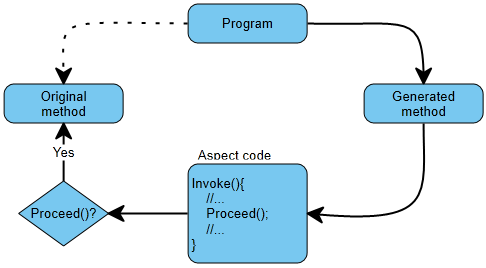
\includegraphics[scale=1.0]{AroundOverview.PNG}
  \centering
  \caption{Method Around Aspect\label{around_overview}}
\end{figure}

The dotted line from Program to the Original method indicates that, once the Around aspect is applied to it, from the perspective of CIL the program cannot directly access that method any more. Access to the original method has to come from inside the aspect. Also note that the original method is not changed at any given time.
